\scanpage{129}
\unsure{ce} groupe $G=\pi/\pi'=\operatorname{Gal}(K/Q)$ opère continûment, et il est engendré topologiquement par les ${}^{\sigma}\overline\tau$ où $\overline\tau\in H$ est l'image de $\tau$, et $\sigma\in G$. Donc il \uline{est annulé par $2$}.

\margin{\figure{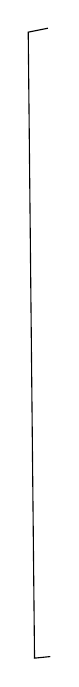
\begin{tikzpicture}\draw (0.25,8)--(0,7.95)--(0.08,0)--(0.28,0.02);\end{tikzpicture}}}
Soit $L$ une extension abélienne de $K$, \deleted{\unsure{son groupe de Gal. $\Gamma$}} son groupe de Galois est donc un quotient $\Gamma$ de $H$; \deleted{Conditions} Supposons $L\ne K$, i.e. $\Gamma\ne\{e\}$. Conditions équivalentes

(i) les $\sigma\tau\sigma^{-1}$ $(\sigma\in\pi)$ coïncident toutes sur $L$ (donc y coïncident avec $\tau:\lambda\to\overline\lambda$)

(ii) $L$ est une extension \uline{quadratique} de $K$ \uline{galoisienne sur} $Q$.

\deleted{\illegible{5}}
\inserted{(iii) $L$ est une extension \uline{quadratique} \uline{purement imaginaire} de $K$.}

De plus, une telle $L$ \deleted{existe et} est unique, [et d'ailleurs existe: il suffit de prendre une extension quadratique imaginaire $E$ de $Q$, \inserted{(p. ex. $Q(\sqrt{-1})$)} et $L=Q(K,E)$ (p. ex. $L=K(\sqrt{-1}))$].

\uline{Dém} (i)$\Rightarrow$(ii) Comme $\Gamma$ est engendré par les images \deleted{\unsure{des}} des ${}^{\sigma}\overline\tau$, \deleted{\unsure{il s}} et que l'hyp. de (i) signifie que ces images sont égales, on voit que (i) implique que $\Gamma$ est engendré par l'élémt $\overline\tau$ de \unsure{expos.} $|2$, donc est $\simeq Z/2Z$ (car $\Gamma\ne(e)$ par hypothèse). D'ailleurs, si un tel $\Gamma$ existe, \deleted{\unsure{il}} \inserted{il est} nécessairement égal à $H_G$ car \deleted{\unsure{lui}} c'est un quotient de $H_G$, et l'argument précédent montre que \deleted{\unsure{ce}} $H_G$ est engendré par un élément d'ordre $|2$. \deleted{\unsure{On}} \deleted{il existe bel et} Il en résulte aussitôt que $L$ est galoisien sur $Q$, donc (i)$\Rightarrow$(ii). D'autre part, (ii)$\Rightarrow$(i), car (ii) implique que $\Gamma\simeq Z/2Z$ \inserted{et que $G$ y opère}, et comme $\Gamma$ est engendré par les images des $\sigma\tau\sigma^{-1}={}^{\sigma}\tau$, i.e. par les ${}^{\sigma}\overline\tau$, on voit que $\overline\tau$ (donc les ${}^{\sigma}\overline\tau$) sont tous égaux à l'unique élément non nul de $\Gamma$.

((i), (ii))$\Longleftrightarrow$(iii) Car du moment que $L$ est quadratique sur $K$, la condition (i) sur les $\sigma\tau\sigma^{-1}$ est évidemment équivalente à (iii)
\mspage{128}
